\subsection{Why learn Data Structures}

\begin{frame}
  \frametitle{Know your data structures!}  There are many types of
  data structures -- You have probably studied all of these
  before. Did you study \structure{how to implement them} or
  \structure{how to use them}?

  {\small
  \begin{block}{Implementation Study -- what you learn?}
    \begin{onlyenv}<1>
      Implement each data structure using the primitives of your
      language.
      \begin{itemize}
      \item What is the time/memory complexity of a data structure?
      \item What kind of bugs can come from a data structure?
      \item How to modify a data structure to fit an specific purpose?
      \end{itemize}
    \end{onlyenv}
  \end{block}

  \begin{block}{Use Study -- what you learn?}
    \begin{onlyenv}<2>
      Apply data structures to various programs using your language's
      API.
      \begin{itemize}
      \item How to dish out a complex data structure quickly;
      \item Which are more or less appropriate to certain problems;
      \item Similarities and differences between them;
      \end{itemize}
    \end{onlyenv}
  \end{block}
  }%\small
\end{frame}

\begin{frame}
  \frametitle{Using the computer's head, not yours}
  {\small
  \begin{columns}[c]
    \column{0.5\textwidth}
    \begin{block}{Time Complexity}
      \begin{itemize}
      \item How fast this algorithm calculates? 
      \item Important for avoiding ``Time Limit Exceeded''. 
      \item Depends on the computer's capacity. 
      \item Faster computers are fast even with slow code.
      \end{itemize}
    \end{block}
    \column{0.5\textwidth}
    \begin{block}{Code Complexity}
      \begin{itemize}
      \item How fast can you debug/modify this code?
      \item Important for avoiding ``Spirit Limit Exceeded''. 
      \item Depends on the programmer capacity. 
      \item Experient programmers understand more complex code.
      \end{itemize}
    \end{block}
  \end{columns}
    }
\end{frame}

\begin{frame}
  \frametitle{Avoiding Code Complexity}

  \begin{itemize}
    \item \structure{Don't reinvent the wheel: learn the API for your
      favorite language;}\\ \only<2>{{\small For Example: stl and
        string for C++; java.util.* for Java; string.h and stdlib.h
        for C.}}
    \item \structure{Before using or implementing a complex method,
      check the size of the problem;}\\ \only<3>{{\small e.g. You want
        to find the highest number in a collection. If the size of the
        collection is smaller than 100, a sequential search might make
        no difference}}
  \end{itemize}

\end{frame}

\subsection{Data Structures}

\begin{frame}
  \frametitle{Data Structure Review}
  \begin{block}{}
    Let's quickly overview some popular Data structures -- you
    probably know all of them.
  \end{block}
  \begin{block}{}
    If you see an ``unfamiliar'' data structure, raise your hand for a
    more detailed explanation.
  \end{block}
\end{frame}

\begin{frame}
  \frametitle{Arrays and Linked Lists}
  \begin{center}
    Implementation infrastructure for all the other types
  \end{center}
  \begin{block}{Arrays}
    \begin{itemize}
    \item Allow random access to any index;
    \item Low code complexity;
    \end{itemize}
  \end{block}
  \begin{block}{Linked List}
    \begin{itemize}
    \item Easy to insert/remove items in the middle;
    \item No predefined size limits;      
    \end{itemize}
  \end{block}

\end{frame}


\begin{frame}
  \frametitle{Stacks}
  \begin{center}
    The simplest data structure.
  \end{center}
  \begin{itemize}
    \item Last-in, First-out policy;
    \item Good on problems where item order is not important;
    \item Also very useful when a \structure{Nested Structure} is necessary:\\
      {\small(Recursion, Counting Parenthesis, Depth First Search)}
  \end{itemize}
  \begin{block}{Common Interface:}
    \begin{itemize}
    \item \structure{Push} -- add a new item to the stack;
    \item \structure{Pop} -- remove the top item from the stack;
    \item \structure{Peek or Top} -- return the top item, but do not remove it;
    \item \structure{Full/Empty} -- return the status of the data structure;
    \end{itemize}
  \end{block}
\end{frame}

\begin{frame}
  \frametitle{Queues}
  \begin{center}
    A ``fairer'' stack, everyone gets their turn.
  \end{center}
  \begin{itemize}
  \item First-In, First-Out policy;
  \item Has some implementation issues:\\
    {\small
    \begin{onlyenv}<2>
      \begin{block}{Stack Implementation}
        Either you have to move all the elements every time you pop an
        item from the queue, or you have to do a ``circular array''
        implementation, keeping track of the first and last items.
      \end{block}
    \end{onlyenv}
    \begin{onlyenv}<3>
      \begin{block}{Linked List Implementation}
        You need to keep a pointer to the start of the list, as well
        as to the end of the list.
      \end{block}
    \end{onlyenv}}
  \item Uses: Deck of cards, Ordered Tasks, Breadth-First Search;
  \end{itemize}
  \begin{block}{Common Interface:}
    Same as stacks (Pop/push/peek), just remember the order policy;
  \end{block}
\end{frame}

\begin{frame}
  \frametitle{POP QUIZ!}
  \begin{block}{How do you implemente a Queue using Stacks?}
    \begin{itemize}
      \item<2->Hint: You need two stacks;
        \bigskip 

      \item<3->Hint: You need an Input Stack and an Output Stack;
        \bigskip

      \item<4>Solution:
        \begin{itemize}
        \item<4> Push all incoming items into the Input Stack;
        \item<4> Whenever you need to pop an item, pop from the Output Stack;
        \item<4> If the output stack is empty, pop every item from the
          input stack and push it into the output stack;
        \end{itemize}
    \end{itemize}
  \end{block}
\end{frame}

\begin{frame}
  \frametitle{Dictionaries}
  \begin{center}
    Data Structure focused on Content, not Position
  \end{center}
  \begin{itemize}
    \item Many different implementations. 
    \item Each different implementation may be more costly to insert,
      delete or search;
    \item Some examples: Sorted Arrays, Binary Trees, Hash tables, etc;
  \end{itemize}
  \begin{block}{Common Interface:}
    \begin{itemize}
    \item \structure{Insert} -- Insert data into the dictionary;
    \item \structure{Delete(x)} -- Delete item with data $x$ from the
      dictionary;
    \item \structure{Search(x)} -- Retrieve an item with content $x$
      from the dictionary;
    \end{itemize}
  \end{block}
\end{frame}

\begin{frame}
  \frametitle{Priority Queue}
  \begin{center}
    A mix of a dictionary/queue, sorted by a value
  \end{center}
  \begin{itemize}
  \item Different kinds of data, tied together by some orderable
    value;
  \item Some examples:\\
    {\small
      \only<2>{(1) Schedule: Which event is next to happen? Prioritize
        by date to happen;}
      \only<3>{(2) Simulation: Similar to scheduling, simulations
        order agents by the next action to be taken;}
      \only<4>{(3) Geometry: Scan algorithms order points based on
        their angles to some location;}
    }
  \item Implementations: Heap, Sorted Array (with extra data for the
    sort value);
  \end{itemize}
  \begin{block}{Common Interface:}
    \begin{itemize}
    \item \structure{Insert, Delete} -- same as dictionary;
    \item \structure{Maximum} -- Get the maximum value in the Priority Queue;
    \item \structure{ExtractMax} -- Get and remove the element with the maximum value;
    \end{itemize}
  \end{block}
\end{frame}

\begin{frame}
  \frametitle{Sets}
  \begin{center}
    A List of Unique Items
  \end{center}

  \begin{itemize}
  \item Order is usually not important;
  \item Elements \structure{NOT} on the Set are as important as the elements in the set;
  \item Implementations: Dictionaries (restrict size!), Bit Arrays, etc;
  \end{itemize}
  \begin{block}{Common Interface:}
    \begin{itemize}
      \item \structure{member(x)} -- does item $x$ belongs to the set?
      \item \structure{union and intersection} -- same as the mathematical operations on sets;
      \item \structure{insert and delete} -- remember that the items are unique!
    \end{itemize}
  \end{block}
\end{frame}

\section{Strings}
\subsection{Strings Representation}

\begin{frame}
  \frametitle{Storing Text}
  \begin{block}{}
    To store text in a computer, we have to transform it into a
    \structure{code} that can be stored into the memory. These codes
    are displayed using associated \structure{Glyphs}.
  \end{block}
  \begin{center}
  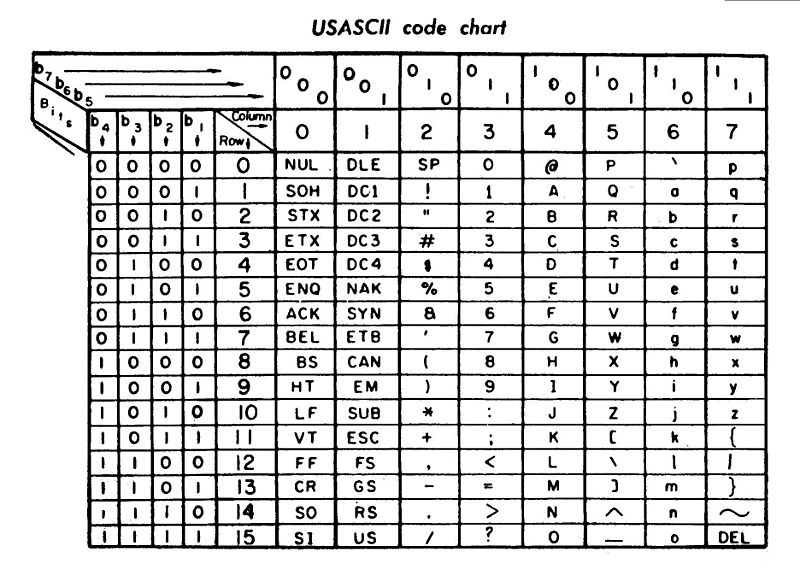
\includegraphics[width=0.6\textwidth]{img/ASCIItableOld}
  \end{center}
\end{frame}

\begin{frame}
  \frametitle{The ASCII Code}
  \begin{columns}[c]
    \column{0.4\textwidth}
    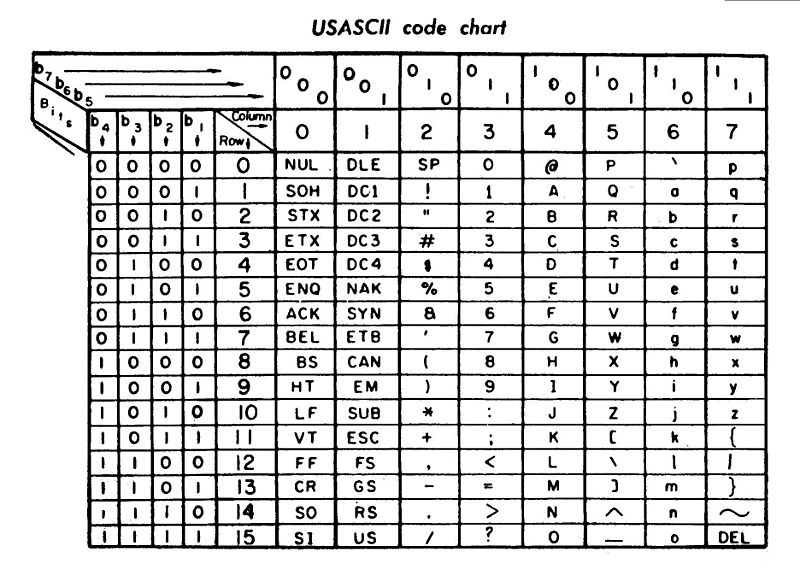
\includegraphics[width=1\textwidth]{img/ASCIItableOld}
    \column{0.6\textwidth}
    \begin{itemize}
      {\small
    \item Each character corresponds to an integer;
    \item The codes corresponding to letters and numbers are in an
      order correspondent to the natural ordering -- you can use a
      code comparison to perform alphabetical comparison.  
    \item There are many other character encodings!
      }
    \end{itemize}
  \end{columns}
\end{frame}

\begin{frame}
  \frametitle{String Representation}
  \begin{center}
    The data structure used to represent strings is usually:
  \end{center}
  \begin{block}{Array representation}
    \begin{itemize}
    \item length value stored at the start of the array;
    \item delimiter value (usually '0') at the end of the array;
    \end{itemize}
  \end{block}
  \begin{block}{Linked List representation}
    \begin{itemize}
    \item same as the linked list we saw at the beginning of the course;
    \end{itemize}
  \end{block}
\end{frame}

\begin{frame}
  \frametitle{String Operations}
  \begin{center}
    These are operations we will often want to perform on a
    string. Which operations are easier/more difficult when using an
    array or linked list?
  \end{center}
  \begin{columns}[c]
    \column{0.5\textwidth}
    \begin{itemize}
    \item Set to a value;
    \item Concatenate strings (``Add'');
    \item Insert substring;
    \item Delete substring (middle, end);
    \end{itemize}
    \column{0.5\textwidth}
    \begin{itemize}
    \item Compare strings;
    \item Find substring;
    \item Change the order of characters (invert, etc);
    \item Search in a string;
    \end{itemize}
  \end{columns}
\end{frame}

